\RequirePackage[hyphens]{url} %Brechen von urls nach spiegelstrichen

\documentclass[a4paper,12pt]{article} %Parameter: twoside
\usepackage[left= 2.5cm, right = 2.5cm, bottom = 4cm]{geometry} %Parameter: showframe
% ============= Dokuinfos =============
\usepackage{hyperref}
\hypersetup{ %https://en.wikibooks.org/wiki/LaTeX/Hyperlinks#Customization
    colorlinks = false, 
    breaklinks, %line breaking in a long hyperlink
    hidelinks,
    urlcolor=green, % farbe von \url
    linkcolor =green, %Farbe von \ref
    citecolor =green, %Farbe von \cite
    linktoc = all %set to all if you want both sections and subsections linked
}

% ============= Packages =============
\usepackage[utf8]{inputenc}
\usepackage[british]{babel} % ngerman
\usepackage[scaled]{helvet} % use helvetica font
\usepackage[T1]{fontenc} %Schriftart
\usepackage{color, xcolor} %colour
\usepackage{float} %big H
\usepackage{pdfpages}

%%Graphikpaket mit Datenpfad
\usepackage{graphicx}
\graphicspath{ {image/} }
\usepackage{caption} %https://en.wikibooks.org/wiki/LaTeX/Floats,_Figures_and_Captions
\usepackage{subcaption} %mehrere Bilder mit Untercaptions
\usepackage{wrapfig}

%Literaturverzeichnis
\usepackage{csquotes}
\usepackage{comment}
\usepackage[ 
% https://www.overleaf.com/learn/latex/Bibliography_management_with_biblatex#Reference_guide
% https://www.overleaf.com/learn/latex/Natbib_citation_styles
% https://www.bibtex.com/e/entry-types/
    backend=biber, % biber backend
    natbib=true, % customising citations
    % sorting=nty, % sort name, title, year
    style=numeric % https://de.overleaf.com/learn/latex/Biblatex_bibliography_styles
]{biblatex}
\addbibresource{references.bib}

%% zusätzliche Schriftzeichen der American Mathematical Society
%\usepackage{amsfonts}
%\usepackage{amsmath}

% ============= zZ Einstellungen/Packages =============
%%Nicht einrücken nach Absatz
\setlength{\parindent}{0pt}

%%Zeilenabstand
\usepackage[onehalfspacing]{setspace} %singlespacing. onehalf-, double-

%%Besondere Trennungen
%\hyphenation{Design-entscheidungen}

%%Weitere  Packages
\usepackage{lipsum} %random Text erstellen mit \lipsum

%%Untertitelanzahl erhöhen
%https://tex.stackexchange.com/questions/186981/is-there-a-subsubsubsection-command

%% Custom Footer with custom page numbering
\usepackage{lastpage}
\usepackage{fancyhdr}
 % Turn on the style
\fancyhf{} % Start with clearing everything in the header and footer

%% Adds new chapter depth
\newcommand{\subsubsubsection}[1]{\paragraph{#1}\mbox{}\\}
\setcounter{secnumdepth}{4}
\setcounter{tocdepth}{4}

%% add new style for listing json
\usepackage{listings}

% ============= First Page edits =============
\usepackage{titling} %Centering
\renewcommand\maketitlehooka{\null\mbox{}\vfill}
\renewcommand\maketitlehookd{\vfill\null}

% needed to set font correctly for the whole document 
\renewcommand\familydefault{\sfdefault} 

\title{Development of an IoT Full Stack System}
\date{6th August 2021}

\begin{document}
    
% ============= Dokumentbeginn =============
\maketitle
\newpage

% Redefine plain style, which is used for titlepage and chapter beginnings
% From https://tex.stackexchange.com/a/30230/828
\fancypagestyle{plain}{%
    \renewcommand{\headrulewidth}{0pt}%
    \fancyhf{}%
    \fancyfoot[L]{\color{gray}{\thepage~|~\pageref*{LastPage}}}%
}
\pagestyle{plain} % activate pagestyle
\setcounter{page}{2} % Seitennummerierung abändern
\tableofcontents %Inhaltsverzeichnis

\newpage

% \newpage
% \listoffigures %Abbildungsverzeichnis
% \listoftables %Tabellenverzeichnis


\section{Motivation}\label{motivation}

The motivation behind this project was to create a system that can take over some gardening work to reduce the time spent on checking on the plants or watering them. The idea is to implement sensors in and around the garden bed to track the surroundings of the plant. \\

Then, with the data from the sensors, it is easier for the user to know when to water the plants or do similar work on the plants. An addition to the sensor is an actuator which can take over simple work on the plant. Watering the plant or controlling the light of an ultraviolet lamp could be some of the tasks that the actuator could take on. And through the collection of data over a longer period of time, the tasks could be done with greater precision. \\

Even when going on a holiday, it would be possible for the user to control this system considering it is connected to the internet. And this is the key motivation. A system to take care of plants or similar objects remotely. \\

%How to realise the vision mentioned above is introduced int he se the scope of this project.




%The motivation behind this project was to have an automated home gardening system so that the user can check on his plants while not being at home and for example water the plants if needed. \\



%This would require to place a sensor in the garden bed that for example measures the moisture of the soil and an actuator which then waters the plants depending on the moisture. \\


\section{Scope of this project}\label{scope}

The goal of this project is to create a frame with which it is possible to have a home gardening system. This means that the whole system has to be modular so that the user can decide which sensors and actuators are needed for the certain situation. \\

The frame consists of three parts which are the webpage or frontend that serves as the human-machine-interface. Then there is the backend that contains the database and the interface for the communication between the frontend to the microcontroller and the backend. And lastly the third part is the microcontroller that processes the data coming from the sensor and actuator. \\

These parts have to work seamingless together ensuring a greater experience when using the system. 


\section{Requirements}\label{req}
This chapter contains the requirements which have been set for this project. The requirements are divided into requirements for frontend, backend and for the microcontroller. These also consider the experience of the project participants for each topic. \\ 

\subsection{Frontend} \label{reqfront}
Considering the requirements for the frontend there are two goals that have to be fullfilled. These are to let the user see all actuator-sensor-pairs (AS-Pairs) in the system and to add any new AS-Pair to the system. \\

A webpage containing a user interface (UI) would be the best choice for these goals. This enables the user to have access on the system from any device and from any place considering that it is connect to the internet. \\

The UI should also be kept simple to ensure a great user experience. The registered AS-Pairs have to stand out and they should be the focus of the webpage. Adding a pair has to be intuitive and self-explanatory. Meaning that it is set what information the user has to add to be able to add an AS-Pair. \\

Further there has to be made a connection between the frontend and the backend. To enable the above mentioned requirements. \\ 

\subsection{Backend and AS-Pair} 

For the subsystem \textit{backend and AS-Pair}, the following requirements are defined:
\begin{itemize}
    \item The subsystem shall be scalable, expandable and maintainable.
    \item For the first implementation, an MQTT interface is to be used.
    \item The AS-Pair should be visualised and controlled by a frontend.
\end{itemize}
\section{Theoretical background}\label{theory}

\subsection{Internet of Things}\label{iot}

The \textit{Internet of Things} (short: IoT) is "the network of physical objects or 'things' embedded with electronics, software, sensors and network connectivity. These objects do collect or exchange data." \cite{iot} This can range from a simple light bulb control via an app to a mesh of sensors in an eg. industrial hall with several monitored machines. The sensors do not have to be in the same place, but can also exchange data globally via the internet.


\subsection{MQTT}\label{mqtt}

The \textit{Message Queuing Telemetry Transport Protocol} (short: MQTT) is a "publish/subscribe messaging protocol [...], that is currently an OASIS [...] standard". \cite{mqtt} This was originally conceived as a lightweight communication protocol for \textit{Machine-to-Machine-communication} (short: M2M-communication) for IoT applications. Due to a low complexity, a high flexibility, low overheads of MQTT packets and the efficient distribution of messages to one or more recipients, MQTT is also suitable for embedded systems and in the communication between networks, applications and middleware. MQTT sends packages over TCP/IP on port 1883 or 8883. \cite{iot} \cite{oasis}\\

MQTT is based on a publish/subscribe model, similar to the Robot Operating System (short: ROS). This means that instead of the classic client-server model, where the client receives a direct response from the server after his request, there is a third system involved which serves as the central distribution system: \textit{The broker}. The broker receives, coordinates and sends all requests to all participants, called \textit{nodes}, subscribed under a so-called \textit{topic}. All nodes can publish or subscribe to a topic. \cite{iot}\\

In principle, this system is comparable to the \textit{Domain Name System} (short: DNS) where the clients make a request under a topic (URL) to a centrally coordinated Server, which resolves this message and forwards it to the requested system. The difference is that there is a known number of registered of IP’s under a URL to which the request needs to be sent. With MQTT, many systems can be notified under one topic, depending on who is subscribed to a topic.\\



\section{Conception}\label{concept}

To reach the scope of this project defined in chapter \ref{scope} an overall system architecture must be designed. The system, seen in figure \ref{fig:fist_conc_system}, consists of three main parts: \textit{Frontend}, \textit{Backend and Database} and \textit{AS-Pair}. The Backend and the Database are connected over an \textit{Interface}.\\

\begin{figure}[H]
    \centering
    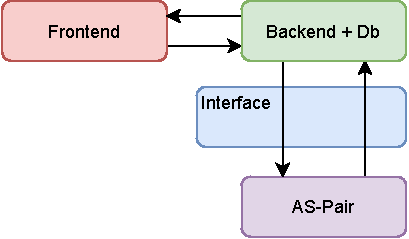
\includegraphics[width=.5\textwidth]{images/4_1/first_concept_ansicht.pdf}
    \caption{Schematic representation of the system}
    \label{fig:fist_conc_system}
\end{figure}

The \textit{Frontend} is the interface where interactions between humans and the rest of the system takes place. It is used to visualise the contents of the database and to control the communication with individual AS-Pairs.\\

The \textit{Backend} serves as a link between the frontend and the AS-Pairs. All interactions and information between the frontend, AS-Pairs and database are routed, controlled and logged via it. The work of the backend is supported by a \textit{database}. This stores information about the system which can be queried at a later time. The database could also be integrated externally.\\

The \textit{AS-Pairs} are the executing link of the system. They handle the messages from the backend, which contain defined commands that are sent via the interface to the AS-Pair. They execute these defined commands depending on the configuration and structure of the AS-Pair.\\

The communication between backend and AS-Pair takes place via an \textit{Interface}. The interface must be supported by both components. The communication between frontend and backend takes place via REST interfaces.\\

The architecture presented offers a high degree of scalability, as standardised interfaces have been used. Furthermore, individual components can be easily replaced or maintained independently of other components without affecting the system as a whole. In addition, task areas are encapsulated, which means that each component fulfils only one specific task. This in turn simplifies the maintenance of these components.\\

In figure \ref{fig:scale_conc_system} one can see the more in detail version of the schematic representation in figure \ref{fig:fist_conc_system}. The character \textit{X} at the end of an enumeration of components stands for an arbitrary number of further systems or components which can be added.

\begin{figure}[H]
    \centering
    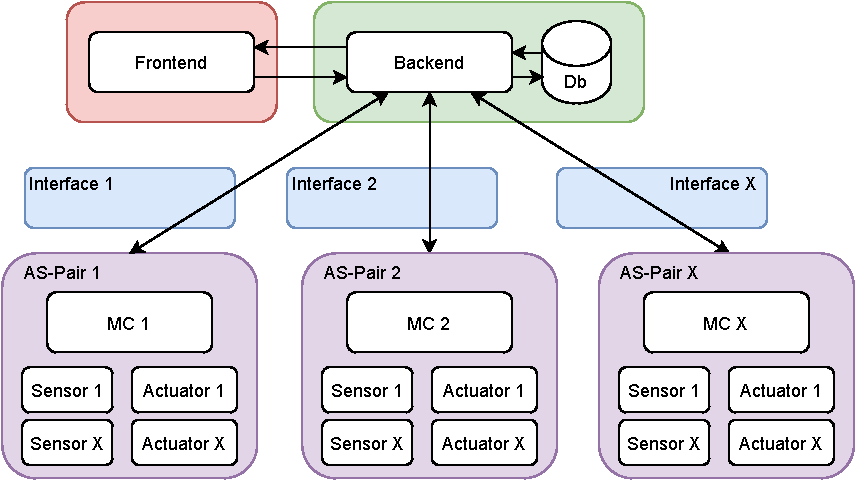
\includegraphics[width=.9\textwidth]{images/4_1/second_concept.pdf}
    \caption{A more detailed schematic representation of the system}
    \label{fig:scale_conc_system}
\end{figure}

For this project, the presented architecture in figure \ref{fig:scale_conc_system} is sufficient. However, if numerous AS-Pairs are required or numerous frontend requests are received, the bottleneck of the system occurs at the backend. If these cases occur, the system would have to be extended with additional backends and additional databases. For this purpose, the system must be extended by load balancers that handle the frontend requests and the communication with the AS pairs and the system can be extended with a database cluster.\\



\subsection{Partially implemented concept}\label{conc_implement}

The overall concept presented in chapter \ref{concept} must now be implemented. For this project, an MQTT interface is used. In figure \ref{fig:mqtt_conc_system} one can see a schematic representation of the overall system with an MQTT interface.\\

\begin{figure}[H]
    \centering
    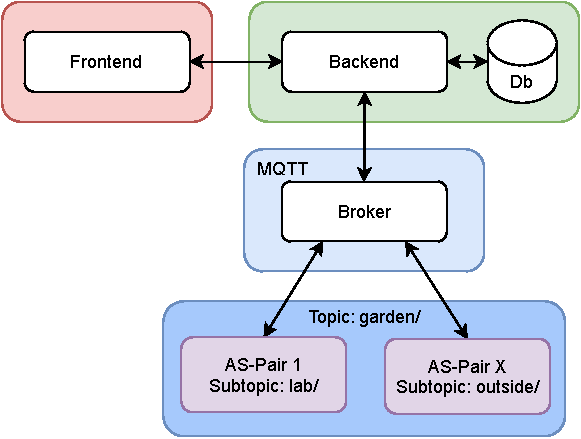
\includegraphics[width=.65\textwidth]{images/4_1/mqtt_concept.pdf}
    \caption{Schematic representation of the system with an MQTT interface}
    \label{fig:mqtt_conc_system}
\end{figure}

For MQTT as an interface, a broker is required for the communication, as described in chapter \ref{theory}.  The broker is located between the backend and AS-Pairs as the central communication system. AS-Pairs that communicate via MQTT can be grouped into different subtopics. In figure \ref{fig:mqtt_conc_system} the AS-Pairs will be grouped under the subtopic \textit{garden/}. Other subtopics can be used for other AS-Pairs subgroups.\\

In this subtopic, different devices can now be differentiated from each other by their own \textit{device topic} like \textit{lab/} or \textit{outside/}. This means that in order to establish communication with eg. AS-Pair 1, one would publish on the topic \textit{garden/lab/}.\\

Thus, AS pairs can be grouped under a special subtask and kept apart eg. by function or place.

\newpage

In figure \ref{fig:hardware_conc_system} one can see the schematic representation of the system which will be used in this project.\\

As already mentioned, this project uses an MQTT interface to communicate with an AS-Pair. The needed broker for an MQTT communication will run on a Raspberry Pi. The frontend, backend and database run on two separate servers.\\

The single AS-Pair, which is addressable under the topic \textit{garden/lab/}, will provide two components, both of which originate from the RWU Board. The potentiometer on channel 0 of the MCP3008 is used as a sensor. The DC motor is used as the actuator, which is controlled via the L239D. An ESP32 forms the middleman between the sensor, the actuator and the MQTT interface to the backend.

\vspace{5mm}
\begin{figure}[H]
    \centering
    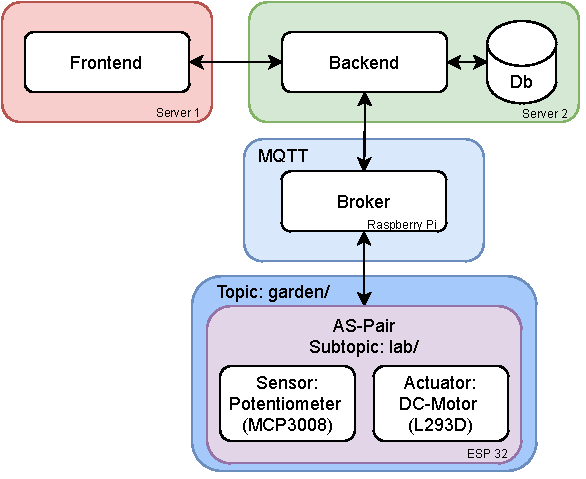
\includegraphics[width=.65\textwidth]{images/4_1/implemented.pdf}
    \caption{Schematic representation of the system used in this project}
    \label{fig:hardware_conc_system}
\end{figure}

\subsection{Backend and AS-Pair}\label{concept_BMC}

This chapter continues to work on the implementation from chapter \ref{conc_implement}. This involves a more in detail implementation of the MQTT interface as well as the backend and the database.

\subsubsection{Database schema}\label{database}

A database is needed to store information in a full stack system. However, this requires a predefined schema, as different schemas come into question depending on the database model, the structure of the data and the querying of the data. In this project, a relational database model will be used for a single backend connection.\\

In order to harmonize the collected data with the system presented in chapter \ref{concept}, the database schema from figure \ref{fig:database_schema} is used.\\

\begin{figure}[H]
    \centering
    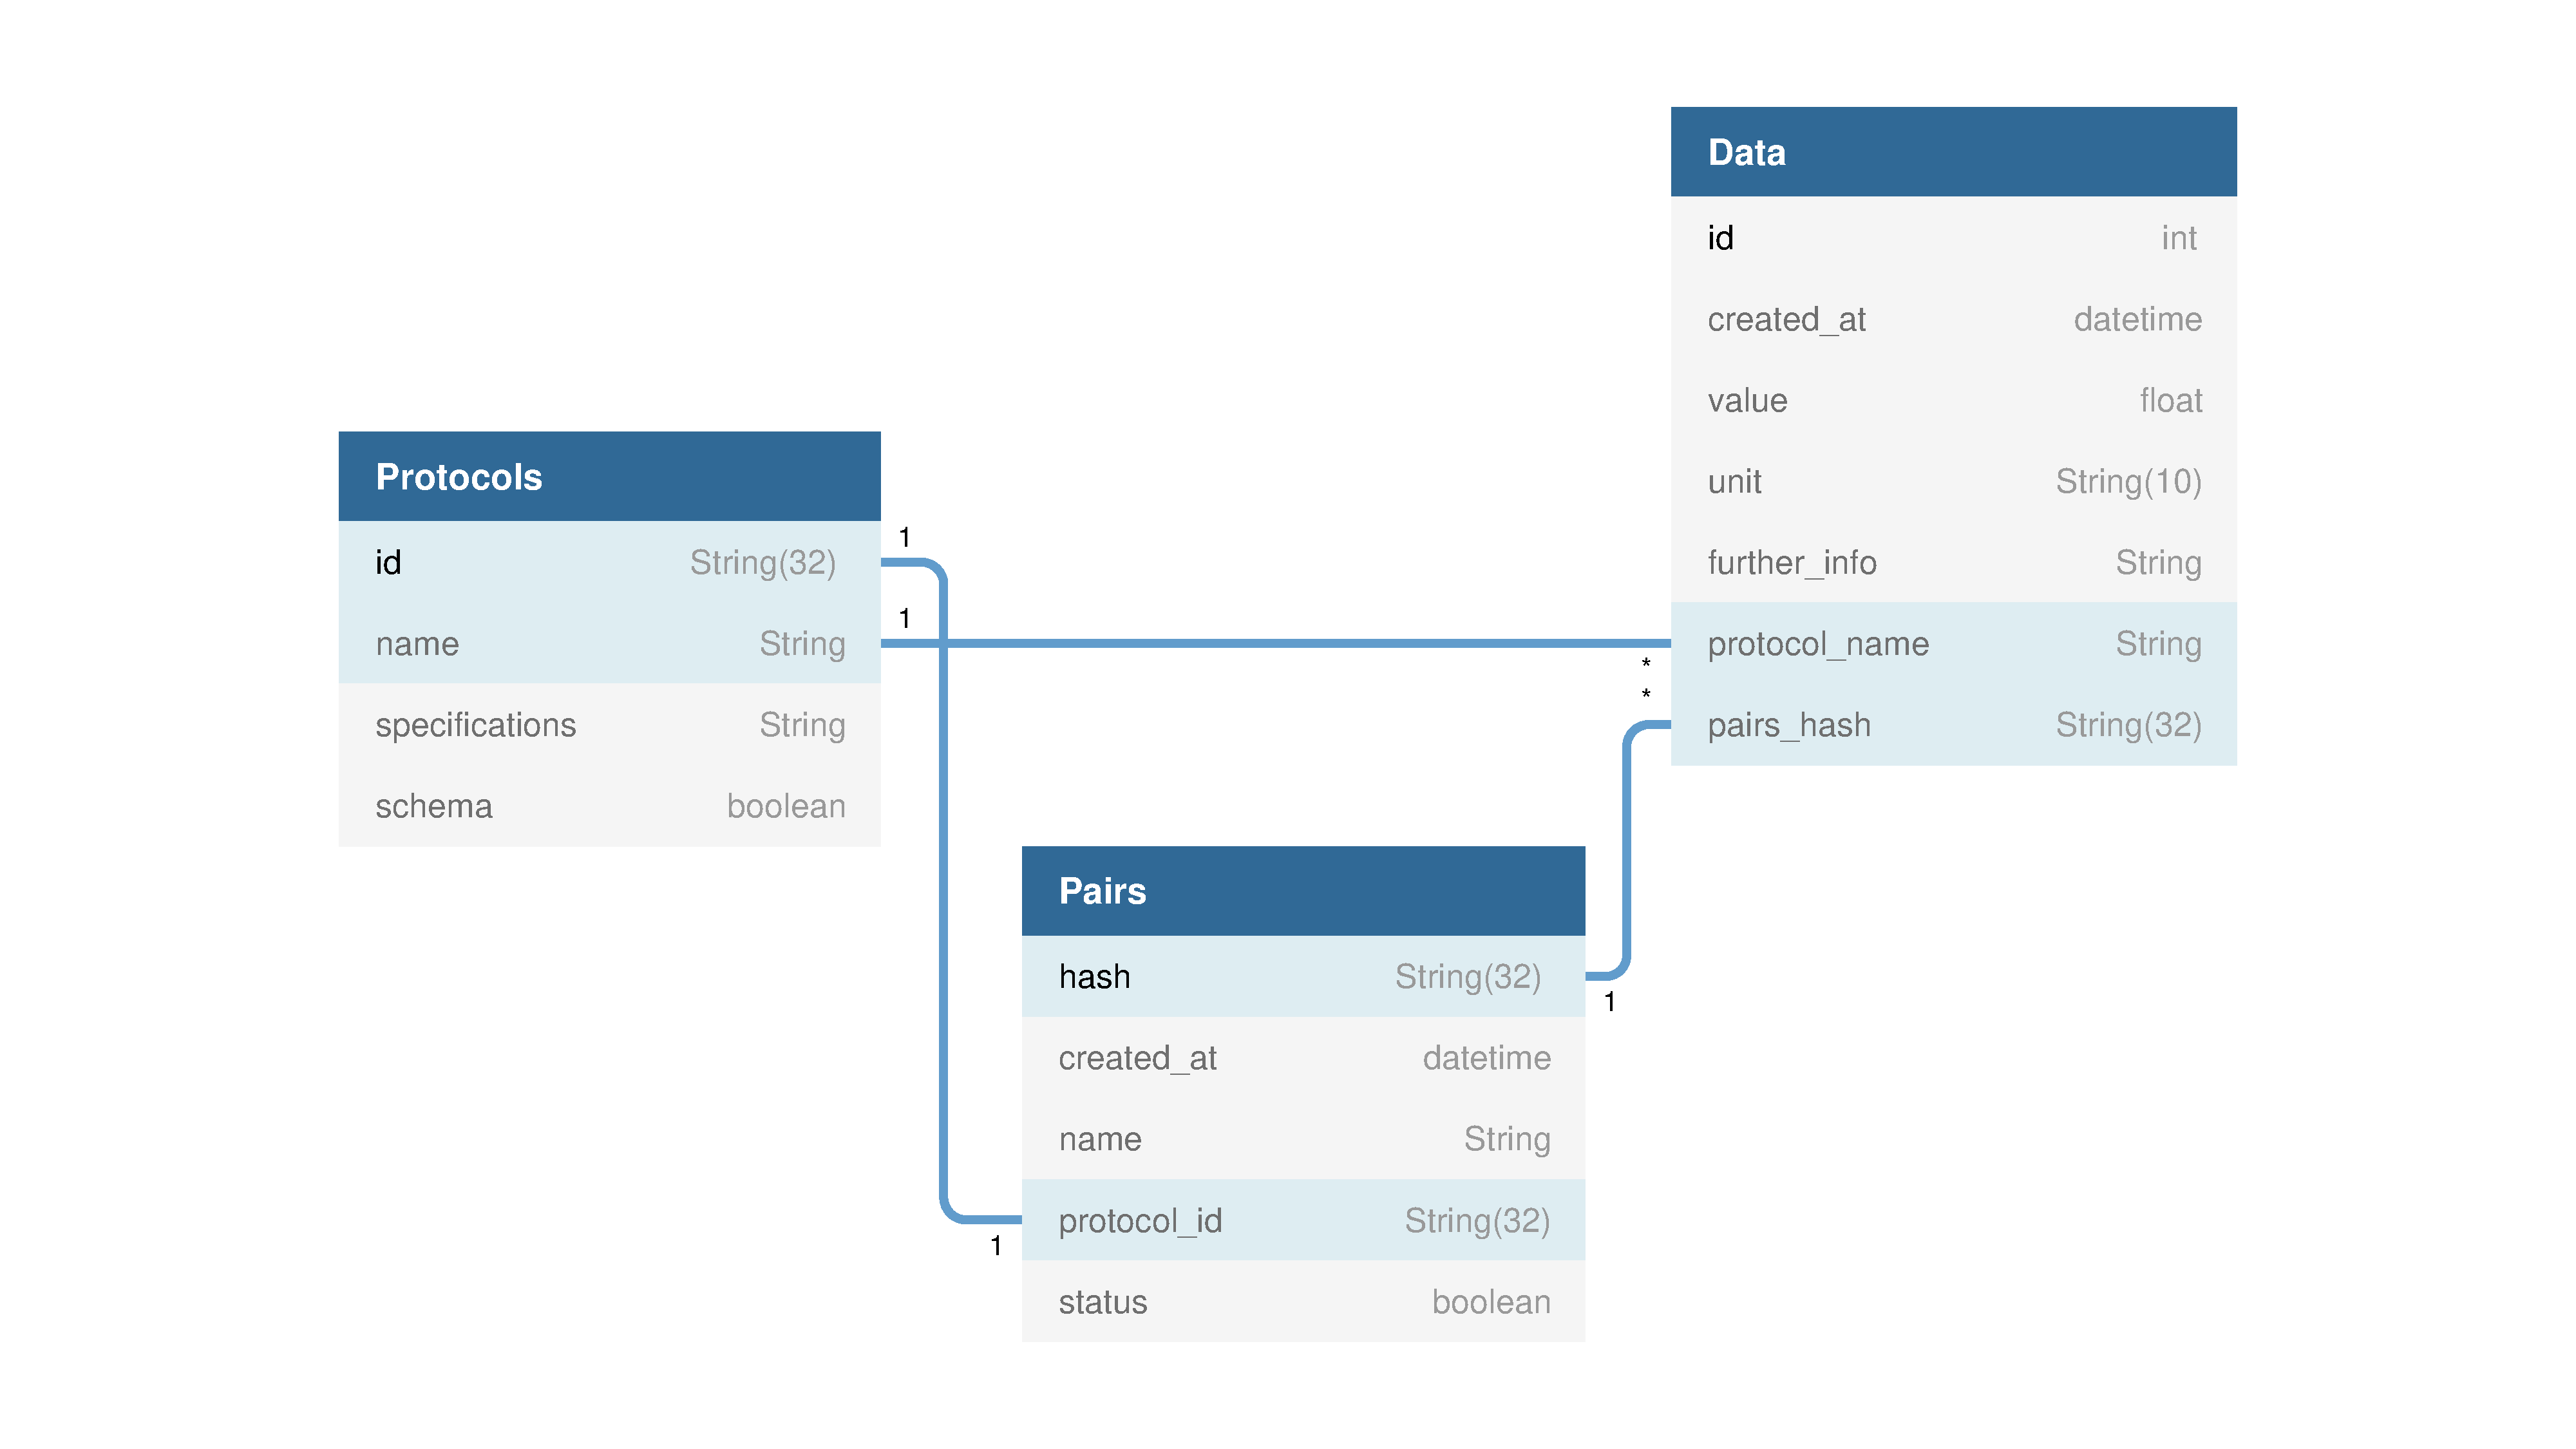
\includegraphics[width=.65\textwidth]{images/4_2/database_schema.pdf}
    \caption{Database schema}
    \label{fig:database_schema}
\end{figure}

Three tables are used for this: \textit{Pairs}, \textit{Protocol} and \textit{Data}. The Protocols and Data tables are assigned to the Pairs table. All registered pairs have a hash as a primary key, which is also stored on the AS-Pair. Each pair has one protocol that stores the parameters under which communication with the pair can take place. Furthermore, the boolean \textit{status} is used to distinguish whether an AS-Pair is still actively accessible via its interface.\\

\newpage

Protocols are again differentiated into registered and schematic protocols via the boolean \textit{schema}. Schematic protocols help the frontend to determine which interfaces are implemented in the backend and which additional information is required by the user to establish a connection to the AS-Pair via this interface. This additional information is stored in the protocol as the string \textit{specifications}. These can be dynamic for each interface.\\

Pairs can have a lot of data. Each data stores a \textit{value} from one sensor per AS-Pair with its \textit{unit} and, depending on how the interface is implemented, dynamically \textit{further information} about the sensor.


\subsubsection{Custom Messages}

MQTT is based on a publish/subscribe model, where data is sent between nodes via a topic to which other nodes are subscribed. It is important to note that data must not be sent on the same topic as the one on which data is received, as this can cause an infinite internal data exchange between nodes. This happens because the broker forwards all incoming data on a topic to all subscribed nodes. If nodes publish and subscribe on the same topic, they receive their own message back from the broker, which they send again on the same topic.\\

To prevent this, a custom messaging schema was developed for this project, which can be seen in figure \ref{fig:custom_msg}.

\begin{figure}[H]
    \centering
    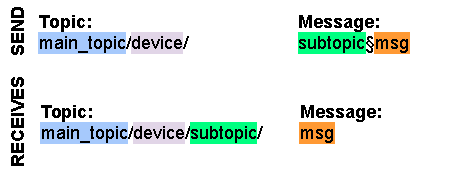
\includegraphics[width=.65\textwidth]{images/4_2/custom_msg.pdf}
    \caption{Custom messaging schema}
    \label{fig:custom_msg}
\end{figure}

If a node or the backend sends a message to another node the \textit{subtopic}, a special command to the AS-Pair which causes a specific reaction of the AS-Pair, is included in the message and separated from a possible message to the AS-Pair via a special character. The node or backend then subscribes to a joined topic, where the subtopic is included.\\

This means that the AS-Pair only has to be subscribed to one topic and can still differentiate all the subtopics sent. The node or the backend can ensure that only the desired AS-Pair will respond to the subtopic that is requested. In figure \ref{fig:custom_msg_ex_1} and figure \ref{fig:custom_msg_ex_2} one can see examples of implemented message exchanges.

\begin{figure}[H]
     \centering
     \captionsetup{justification=centering}
     \begin{minipage}[b]{0.5\textwidth}
         \centering
         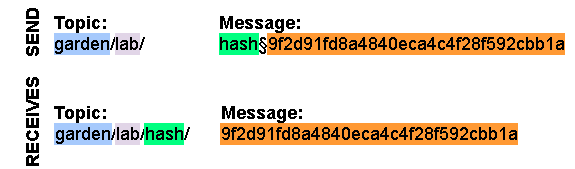
\includegraphics[width=\textwidth]{images/4_2/custom_example_1.pdf}
         \caption{Custom messages - Example 1}
         \label{fig:custom_msg_ex_1}
     \end{minipage}%
     \begin{minipage}[b]{0.5\textwidth}
         \centering
         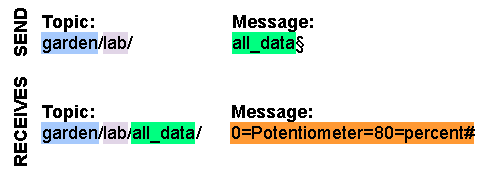
\includegraphics[width=\textwidth]{images/4_2/custom_example_2.pdf}
         \caption{Custom messages - Example 2}
         \label{fig:custom_msg_ex_2}
     \end{minipage}
\end{figure}


Figure \ref{fig:custom_msg_ex_2} is an example if several pieces of information have to be kept apart. In this case, information from sensors is decoded in a special pattern and sent to the requesting node or backend. The individual information and the individual information of the components are separated via special separating characters. It must be ensured that special separating characters are used that do not occur in possible values. The formatting of the message is the responsibility of the programmer of the interface.\\

In this example, information is requested from all sensors. The message received follows a strict specification: Individual sensors are separated via the \textit{\#}-character. In the segments, the ID of the sensor, its name, its value and its unit are then concatenated via the \textit{=}-character.\\

The same scheme is used to obtain all information about the implemented actuators. However, the content of the segments changes. The ID of the actuator, its name and its possible changeable variables with their data type are in this case returned.

\subsubsection{Routes}

For this project, 4 main workflows are to be implemented:  \textit{hash\_init}, \textit{get\_all\_data},\\ \textit{get\_actuator\_data} and \textit{set\_actuator}. These are shown and explained in the following figures.
\newpage

\begin{wrapfigure}{L}{0.55\textwidth}
    \centering
     \captionsetup{justification=centering}
     \begin{minipage}[b]{0.53\textwidth}
         \centering
         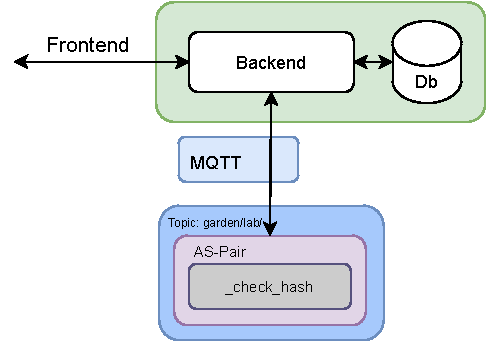
\includegraphics[width=\textwidth]{images/4_2_1/hash_init.pdf}
         \caption{Workflow \textit{hash\_init}}
         \label{fig:hash_init}
     \end{minipage}
     \vspace{-.25\baselineskip}
\end{wrapfigure}

\subsubsubsection{Initialize Hash}

In figure \ref{fig:hash_init} one can see the workflow of the \textit{hash\_init} route. The aim of this workflow is to register an AS-Pair in the backend.\\

For this purpose, the frontend sends a request to the backend with information about the AS-Pair, such as its name, which interface is to be used and what information is needed to establish a connection with the AS-Pair. For MQTT, this would be the IP of the broker and the topic of the AS-Pair. This allows the backend to attempt to establish communication with the AS-Pair. \\

The Backend, however, checks beforehand whether there is already a similar AS-Pair in the database. If such an AS-Pair with the given specifications is already specified in the database, it is reactivated if it if no connection has been established in a longer period of time, i.e. its flag \textit{status} is set to True, or a message is returned to the frontend that the sent AS-Pair already exists and is active. This avoids duplicate entries from the same AS pair.\\

If a communication has been successfully established with the AS-Pair under the subtopic hash, the AS-Pair checks whether it has already saved a hash. For this purpose, it receives from the backend either a newly generated hash, if no database entry exists, or an already registered hash, if an entry in the database exist with the same specifications.\\

If the AS-Pair was able to save the hash successfully, positive feedback is sent back with the hash as the message, which the backend stores with all relevant data in the database and sends a positive message back to the frontend.\\

\begin{wrapfigure}{L}{0.43\textwidth}
    \centering
     \captionsetup{justification=centering}
     \begin{minipage}[b]{0.39\textwidth}
         \centering
         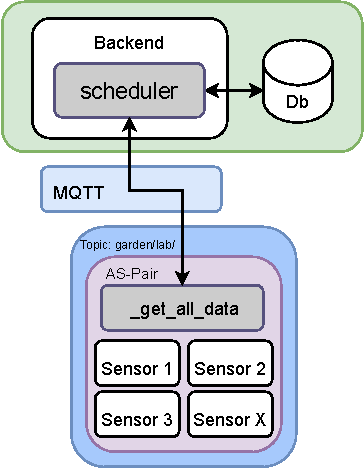
\includegraphics[width=\textwidth]{images/4_2_1/scheduler_all_data.pdf}
         \caption{Workflow \textit{get\_all\_data}}
         \label{fig:schedule}
     \end{minipage}
     \vspace{-.25\baselineskip}
\end{wrapfigure}

\newpage

\subsubsubsection{Scheduler}

In figure \ref{fig:schedule} one can see the workflow of the \textit{hash\_init} route. The aim of this workflow is to store the value from all initialized sensors of all registered AS-Pairs in the database at periodic intervals.\\

For this purpose, the backend needs a scheduled task that queries all active AS-Pairs from the database in a fixed interval and attempts to establish a communication with this AS-Pairs over their specified communication specifications. \\

Since numerous AS-Pairs can be registered and individual requests may exceed the interval time, depending on the selected interval time, these communications must take place in asynchronous threads. This way, individual requests do not block each other and several requests can be processed simultaneously over the I/O Interfaces.\\

These requests are made under the subtopic \textit{data\_all} to all active AS-Pairs. Through this subtopic, the AS-pair returns all data from all initialized sensors. The developer of the interface can decide how he wants to save the result of the sensors into the database through the column \textit{further information}. However, two values must be stored per data-row in the table data, i.e. per sensor: The value of the sensor and the unit of this value.\\

\begin{wrapfigure}{L}{0.43\textwidth}
    \vspace{\baselineskip}
    \centering
     \captionsetup{justification=centering}
     \vspace{-4mm}
     \begin{minipage}[b]{0.39\textwidth}
         \centering
         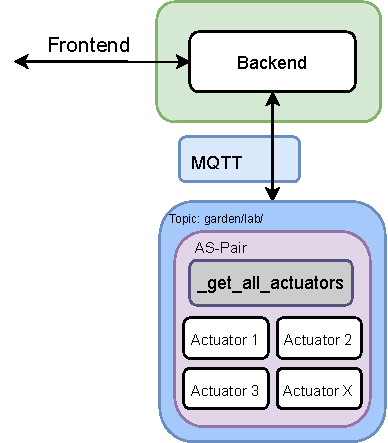
\includegraphics[width=\textwidth]{images/4_2_1/get_actuator.pdf}
         \caption{Workflow \textit{get\_actuator\_data}}
         \label{fig:get_act}\par
         \vspace{9mm}
         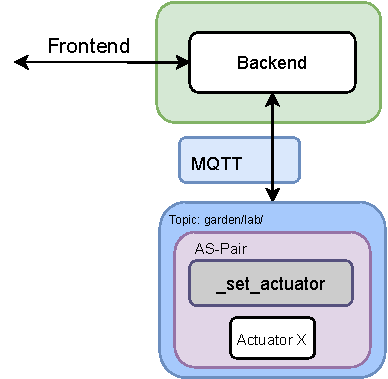
\includegraphics[width=\textwidth]{images/4_2_1/set_actuator.pdf}
         \caption{Workflow \\\textit{set\_actuator}}
         \label{fig:set_act}
     \end{minipage}
     \vspace{-.25\baselineskip}
\end{wrapfigure}

\subsubsubsection{Get and set Actuator}

In figure \ref{fig:get_act} and \ref{fig:set_act} one can see the workflows of the \textit{get\_actuator\_data} and \textit{set\_actuator}. The aim of the overall workflow is to control a registered Actuator of an AS-Pair. This requires information about the actuators and their changeable variables, as well as an interface with which a specific actuator can be controlled.\\

\newpage

For this purpose, the frontend sends a request to the backend with information about which AS-Pair it would like to receive information about its actuators. The backend sends a request via the interface under the subtopic \textit{actuator\_all} to the specified AS-Pair.\\

The AS-pair sends back a list of all initialized actuators in a special way: ID of the actuator, its name and its possible changeable variables with their data type. The changeable variables depend on the implementation of the actuator. \\

This information is sent back to the frontend. From this information, the frontend or the user can now send a request to the backend to change the variables mentioned in the reply.\\

For this purpose, the frontend sends a message to the backend with the information which actuator ID is to be controlled at which AS-Pair and the variables with their new values.\\

The backend communicates with the specified AS-Pair via it's interface and communicates the new information. If the actuator was successfully controlled with the new values, the AS-Pair sends a positive message to the backend, which returns a positive message to the frontend. \\

In the event of an error, the error message is communicated to the frontend via the backend.


\subsection{Frontend}\label{concept_fron}
Considering the frontend of the project first there has to be a design which fits to the requirements mentioned in the chapter \ref{reqfront}. This design shows in a more broad way how the features of showing AS-Pairs and adding AS-Pairs are implemented. \\

\subsubsection{Design Concept of the webpage}

\begin{figure}[H]
    \centering
    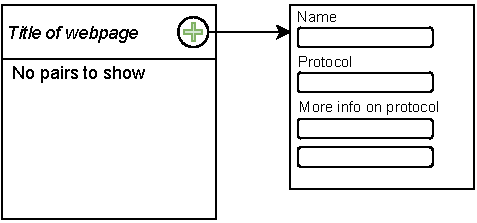
\includegraphics[width=.65\textwidth]{images/4_3/concept-webpage.pdf}
    \caption{Concept of the webpage}
    \label{fig:concept-webpage}
\end{figure}

Figure \ref{fig:concept-webpage} shows the concept of how the webpage should look like. The window on the left side is the first thing the user should see. It contains the title of the webpage, a plus sign button that holds the function to add pairs and the pairs that are in the database. For the case in figure \ref{fig:concept-webpage} there are no pairs in the database which is the reason why a default text is presented to the user informing him that no pairs are available. \\

If the user then clicks on the plus sign button it should bring up the window seen on the right side of figure \ref{fig:concept-webpage}. There information is needed from the user to be able to add an AS-Pair to the database. \\

The user has to first name the AS-Pair then the protocol has to be selected. In this case the protocol would be MQTT but the types of protocols can be anything an not only MQTT. To establish a connection between the AS-Pairs and the backend it is necessary to specify the IP of the broker and to which topic and subtopic the new AS-Pair belongs to. \newpage

\begin{wrapfigure}{L}{0.5\textwidth}
    \centering
     \begin{minipage}[b]{0.5\textwidth}
         \centering
         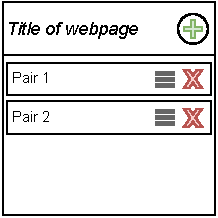
\includegraphics[width=\textwidth]{images/4_3/concept-webpage-pairs.pdf}
         \caption{Concept of the webpage with added AS-Pair}
         \label{fig:concept-webpage-pairs}
     \end{minipage}
  
\end{wrapfigure}

Only when the correct information has been entered by the user then it is possible to save the AS-Pair in the database. Which then would show up on the webpage. An example can be seen in the figure \ref{fig:concept-webpage-pairs} where pairs are available in the database. \\

As an addition there have been buttons added to delete a pair (red X button) and to show more information about the pair (three bars button) for further improvement of the webpage and the system interaction. But these buttons won't have any function for now as they are not important for the requirements. \\

\subsubsection{Realization of the Design Concept}

Now that the concept of the design is set it has to be realized. This is done through a JavaScript library called \textit{React.js}. Normally when building a user interface for a webpage it would need to implement HTML, CSS and JavaScript. With React the whole UI is made in one JavaScript file. That makes for a great benefit as it is now simpler to create an UI on a webpage. \\

Another benefit of React is that it optimizes the rendering of the web application which in turn has a benefit on the speed of the web application. This is done through taking the most recent domain object model (DOM) which is a tree like structure of all HTML-elements and creating a virtual DOM. When there are changes on the webpage it only compares the current state with the one that is saved as the virtual DOM. Then only the certain parts that are different will be rendered instead of calculating every CSS- and HTML-Element anew on the webpage when there have been changes made. \newpage

When creating the webpage as envisioned in the concept it is better to divide it into different parts as it reduces the complexity. These parts would for example be the \textit{Add-Button} or the \textit{Add-Pair-Form}. This is easily applicable in React and is even a feature that stands out as they are called components. Components are just reusable parts of the UI. \\

These components are separate JavaScript files that are then included in the main JavaScript file that renders the whole UI. Each of these components for the realization of the concept can be seen in figure \ref{fig:components} where they are highlighted.\\

\begin{wrapfigure}{r}{0.5\textwidth}
    \centering
     \begin{minipage}[b]{0.5\textwidth}
         \centering
         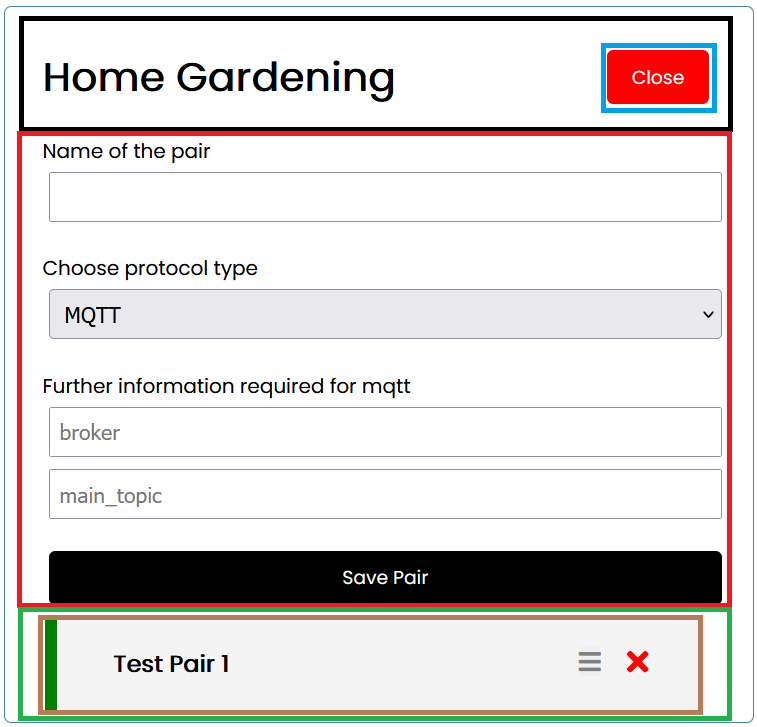
\includegraphics[width=\textwidth]{images/4_3/components.png}
         \caption{Components of the UI}
         \label{fig:components}
     \end{minipage}
     \vspace{-.25\baselineskip}
\end{wrapfigure}

The black border shows the \textit{header} component which contains the title of the page in this case \textit{Home Gardening} and the button component \textit{close}. The function of that button is to show and hide the form to add a new pair to the system. \\

With it being a component it is possible to pass so called properties, which are attributes that hold values. These props are used to change the color of the button or to change the text inside of it depending on if the form is shown or not. \\

Through the component highlighted in the red rectangle it is possible for the user to add a new pair. This component shows the user a form where different values are asked that resemble the idea in the conception of adding a new pair. \\

The name, protocol type and the information to connect to the protocol are needed which will be passed into a function in the main JavaScript file as a prop. This function handles the values received from the \textit{add-pair-form} component and passes them to the backend. \newpage

To pass values to the backend a POST-Request has to be made which is a HTTP-Request. This enables the communication between the server of the frontend and the server of the backend. \\

A successful communication is only possible if the user has stated the correct \textit{broker} and \textit{main topic} of the MQTT Protocol for example. To show the pairs that are available in the database the component in the green rectangle is created. That also contains another component for each individual pair. \\ 

To retrieve data about the pairs in the database and to display them on the webapp another HTTP-Request has to be done called \textit{GET}. These pairs are then saved in an object where through a \textit{map}-function every single pair is read and rendered onto the webpage as seen in the green rectangle in figure \ref{fig:components}. \\

\begin{figure}[H]
    \centering
    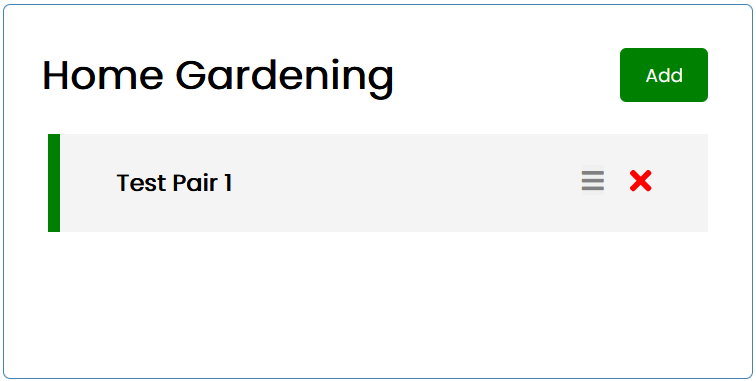
\includegraphics[width=.65\textwidth]{images/4_3/Screenshot 2021-07-27 095812.png}
    \caption{UI with an AS-Pair}
    \label{fig:UI-AS-Pair}
\end{figure}

Figure \ref{fig:UI-AS-Pair} shows how the webapp is rendered without the Add-Pair-Form being visible. Each pair shows the name of the pair and the status through the green bar on the left side of the pair. Additionally a \textit{red X button} and a button resembled by three bars are visible inside the pair component. \\

Even though the buttons are displayed they don't have any function but this satisfies the concept which also shows a \textit{red X button} and a \textit{three bars button}. These have already been implemented to later add a function to them.










%\section{Test of the developed components}

\begin{wrapfigure}[19]{L}{0.43\textwidth}
    \vspace{-\baselineskip}
    \centering
     \begin{minipage}[b]{0.39\textwidth}
         \centering
         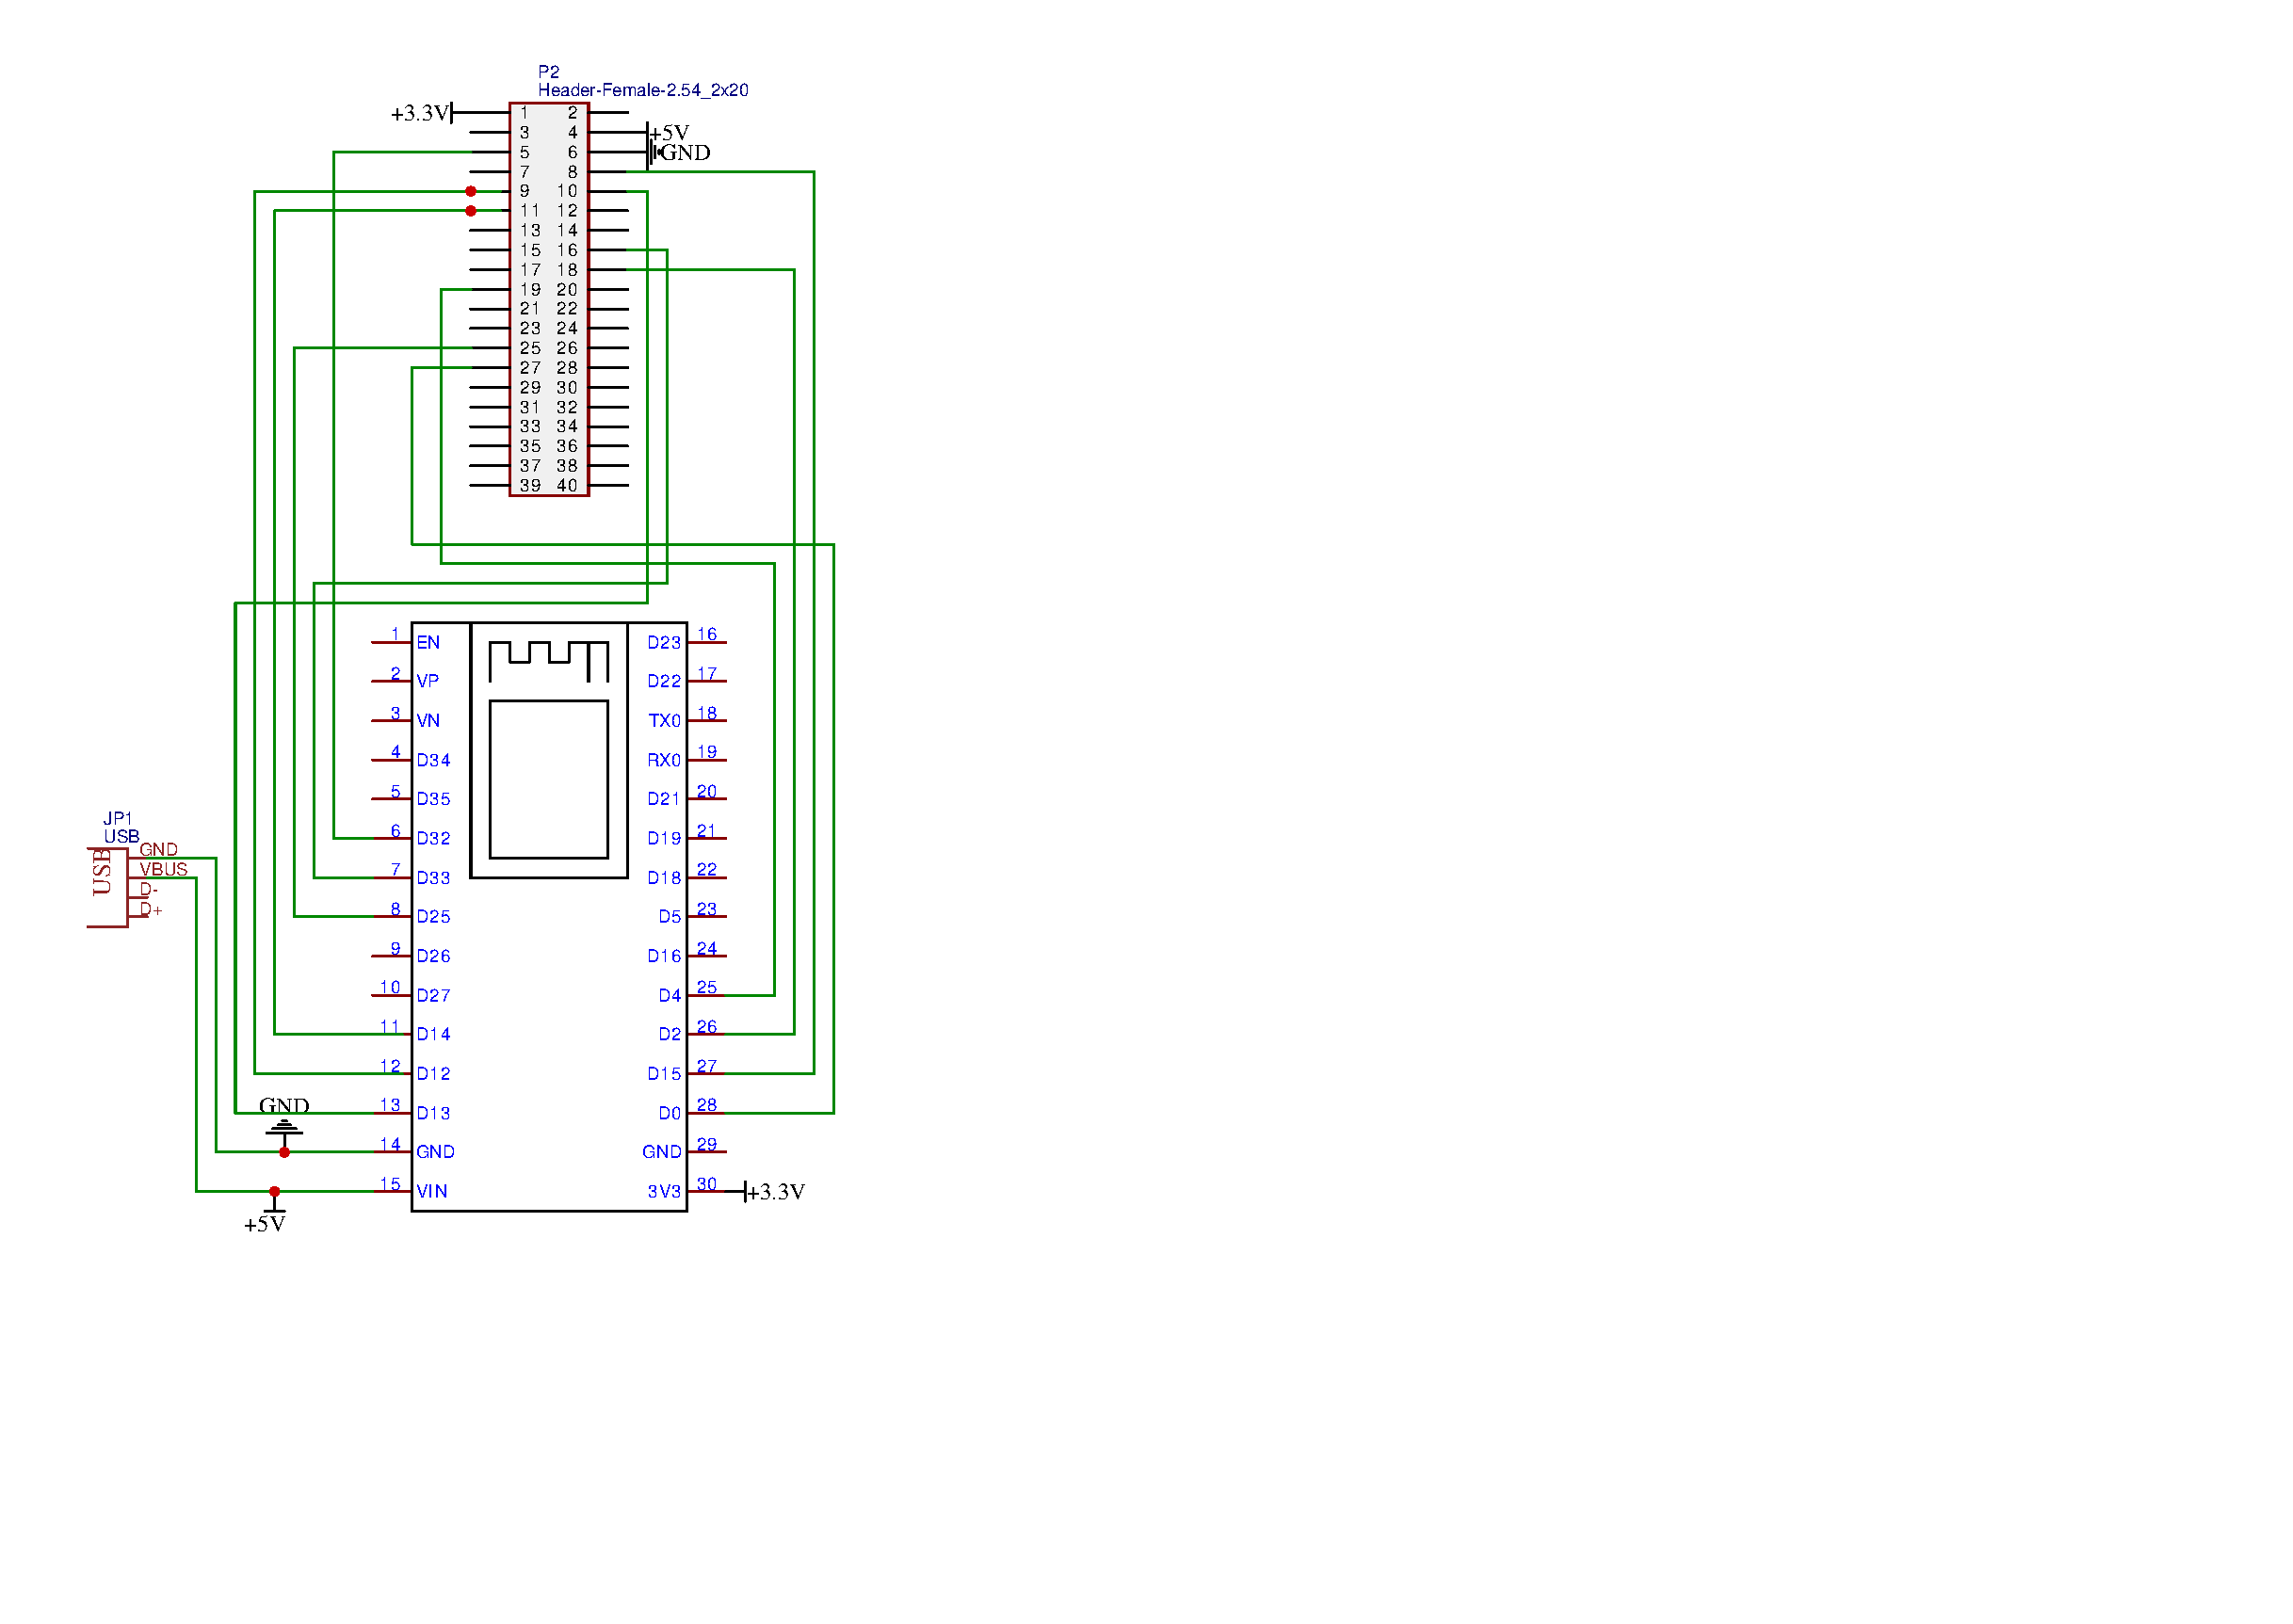
\includegraphics[width=\textwidth]{images/4_2/schmatic_project.pdf}
         \caption{Electrical diagram}
         \label{fig:schem_electronics}
     \end{minipage}
     \vspace{-.25\baselineskip}
\end{wrapfigure}

In this chapter, the conceptual design of chapter \ref{concept} is used. It must be considered that only systems and routines that have been implemented in all three components, i.e. in the frontend, in the backend and in the AS-Pair, will be presented.\\

One can see in figure \ref{fig:schem_electronics} the electronic connections drawn from the ESP32 to the Raspberry GPIO interface of the RWU board.\\

\vspace{4cm}

\begin{listing}[H]
    \begin{minted}[frame=single,
                   framesep=3mm,
                   linenos=true,
                   xleftmargin=21pt,
                   tabsize=3]{json}
{
    "name": "Love_Ship",
    "protocol": {
			"name": "MQTT",
			"specifications": {
				"broker": "192.168.4.1",
				"main_topic": "garden/lab"
			}
		}
}
    \end{minted}
    \vspace{-4mm}
    \caption{Adding an AS-Pair} 
    \label{list:adding_pair}
\end{listing}

\section{Conclusion}\label{summary}

The initial objective in chapter \ref{scope} has been successfully achieved. A system was implemented that allows the user to add sensors, actuators and AS-Pairs in a modular way. This information is stored in a database and displayed on a frontend.\\

Furthermore, the defined requirements in chapter \ref{req} were also successfully implemented. New AS-Pairs can be added via a UI on a website. The UI is simple and minimalistic. The frontend communicates with the backend and are coordinated with each other. The backend is scalable in the number of AS-Pairs and can communicate with them via any number of implemented interfaces. \\

The AS-Pair is scalable in the number of sensors and actuators which can be implemented. These communicate with the backend via MQTT. The interfaces of the AS-Pairs can be accessed via the frontend. Due to the selected system architecture, all components are separated from each other and thus simplify maintainability.\\

However, the system can be extended by some points in further versions. The frontend can extend the UI with further functions, such as deleting an AS-Pair and visualising the accumulated data in the database per AS-Pair. Furthermore, the communication paths between the three components needs to be encrypted, so that sensitive data cannot be intercepted, and the individual components need to be protected against attacks.



\sloppy %Toleranzen setzen
\printbibliography[heading=bibintoc]
%\printbibliography[heading=bibintoc, keyword=pic, title={Pictures only}]
\fussy %Toleranzen zurücksetzen



\end{document}
